% Resumo no template ISMIR 2026 (ismir.sty, cite.sty e cc_by.* copiados de github.com/ismir/paper_templates).
\documentclass{article}
\usepackage[T1]{fontenc}
\usepackage[utf8]{inputenc}
\usepackage[brazilian]{babel}
\usepackage{ismir} % sem a opção "submission": a entrega não é anônima
\usepackage{amsmath,cite,url}
\usepackage{graphicx}

\title{Bossa Nova no Estilo de Jobim com Cadeias de Markov de Harmonia e Contorno}

\oneauthor
  {Victor Yuji Yano}
  {\texttt{victoryujiyano@gmail.com}}

\def\authorname{V. Y. Yano}

\sloppy

\begin{document}

\maketitle

\begin{abstract}
Geramos peças de bossa nova no estilo de Tom Jobim com duas cadeias de Markov de ordem $n$ aprendidas do MPB Corpus: uma sobre acordes e outra sobre o contorno melódico. Analisamos o compromisso entre ordem e memorização.
\end{abstract}

\section{Introdução}
Cadeias de Markov são um método clássico de composição algorítmica~\cite{pachet2003}. Usamos exclusivamente esse método, com a restrição estilística de \emph{bossa nova no estilo de Tom Jobim}.

\section{Trabalhos relacionados}
Pachet~\cite{pachet2003} propõe Markov de ordem variável para improvisação interativa; Conklin~\cite{conklin2003} revisa modelos estatísticos para música, incluindo $n$-gramas. O MPB Corpus~\cite{mpb} fornece anotações simbólicas de 500 canções brasileiras, base dos nossos modelos.

\section{Método}
\textbf{Corpus.} 50 composições de Jobim do MPB Corpus (CC BY 4.0). O corpus não contém MIDI nem alturas absolutas: usamos \texttt{harmony.csv} (raiz, tipo de acorde e compasso de entrada; 49 trechos em modo maior e 21 em menor) e as letras de contorno de \texttt{contour\_rhythm.csv} ($u$ repete; $P/p$ grau conjunto acima/abaixo; $A/a$ arpejo de 3--5 semitons; $S/s$ salto $\ge 6$).

\textbf{Harmonia.} Estado $(\text{raiz}-\text{tônica},\text{símbolo},\text{duração})$, com duração em $\{0{,}5;1;2;4\}$ compassos; saída em Dó maior ou Lá menor.

\textbf{Melodia.} Cadeia sobre as letras de contorno, com um separador de frases. Cada frase começa num tom do acorde vigente e as letras são decodificadas em notas (graus conjuntos na escala; arpejos e saltos preferindo tons do acorde). O ritmo da melodia não é decodificável a partir do corpus; usamos um ciclo sincopado fixo (decisão nossa).

\textbf{Acompanhamento.} Camada de renderização por regras, fora do modelo de Markov: baixo (raiz/quinta) e violão na clave de bossa 3-2.

\textbf{Probabilidades e ordem.} As probabilidades de transição são aprendidas por contagem no corpus, com \emph{backoff} para ordens menores quando o contexto não existe. Hiperparâmetros: modo, ordem da harmonia, ordem do contorno e semente. Usamos $n=2$--$3$ na harmonia e $n=3$--$4$ no contorno (justificativa na Seção~\ref{sec:res}). As peças têm 32 compassos a 132~bpm e são exportadas em MIDI.

\section{Resultados}\label{sec:res}
Geramos 5 peças variando modo, ordens e sementes (arquivos 	exttt{jobim\_*} em 	exttt{music/}): 	exttt{major\_h2\_m3\_seed1} e 	exttt{major\_h2\_m3\_seed2} (mesma configuração, sementes diferentes), \texttt{major\_h3\_m4\_seed3}, \texttt{minor\_h2\_m3\_seed4} e \texttt{minor\_h3\_m3\_seed5}, em que 	exttt{h} e 	exttt{m} são as ordens da harmonia e do contorno.

Medimos a fração da sequência gerada que é cópia literal de um trecho do corpus (15 sementes por ordem; Fig.~\ref{fig:order}). Na harmonia, a cópia sobe de 0,18 ($n=1$) para 0,53 ($n=2$), 0,67 ($n=3$) e 0,81 ($n=6$); no contorno, de 0,12 para 0,14 ($n=3$) e 0,39 ($n=6$).

\begin{figure}[t]
\centering
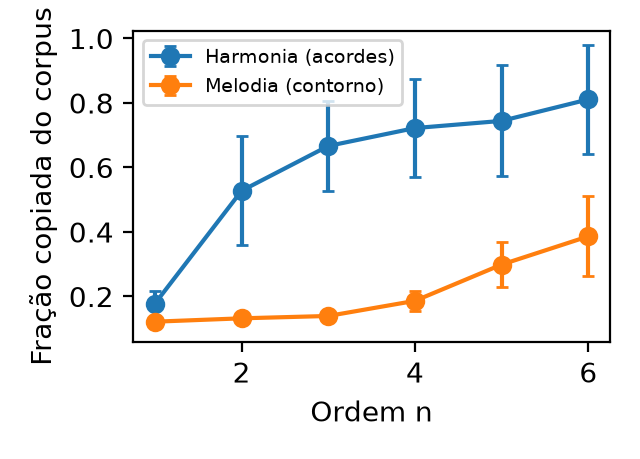
\includegraphics[width=\columnwidth]{order_vs_copy.png}
\caption{Fração copiada do corpus vs. ordem (média $\pm$ desvio).}
\label{fig:order}
\end{figure}

\textbf{Trade-off da ordem.} Ordens baixas geram material mais genérico e menos idiomático; ordens altas são mais fiéis ao corpus, mas passam a memorizar trechos inteiros. O corpus de harmonia é pequeno (1\,837 acordes em maior) e o estado inclui a duração, então já com $n=2$ mais da metade da sequência é cópia. Por isso escolhemos $n=2$--$3$ na harmonia. O alfabeto do contorno tem poucos símbolos, e é preciso $n=3$--$4$ para capturar motivos sem copiar (14--19\% de cópia).

\textbf{Observações.} Cada peça tem de 34 a 46 acordes (14 a 19 tipos distintos) e de 84 a 90 notas de melodia, em extensões de 12 a 19 semitons. Entre 49\% e 77\% das notas da melodia pertencem ao acorde vigente, o que mantém a melodia coerente com a harmonia, mas deixa o restante a cargo de passagens por grau conjunto. As progressões incluem ciclos típicos de Jobim, como \emph{m7} seguido de dominante \emph{7(b9)} ou \emph{7.13}. % TODO: acrescente aqui suas impressões de audição (1-2 frases).

\section{Discussão e trabalhos futuros}
Limitações: a melodia é pobre ritmicamente; melodia e harmonia são cadeias independentes, ligadas só na decodificação; o acompanhamento é baseado em regras; a síntese é simples. Futuro: obter alturas e ritmos de partituras de Jobim, condicionar a melodia ao acorde e avaliar com ouvintes.

\begin{thebibliography}{9}
\bibitem{pachet2003} F.~Pachet. The Continuator: Musical Interaction With Style. \emph{Journal of New Music Research}, 32(3):333--341, 2003.
\bibitem{conklin2003} D.~Conklin. Music Generation from Statistical Models. In \emph{Proc. AISB Symposium on AI and Creativity in the Arts and Science}, 2003.
\bibitem{mpb} Almada, Carvalho and Martins. The MPB Corpus: A Dataset of Melody, Rhythm, Harmony, and Melody-Harmony Relationships in Brazilian Popular Music. arXiv:2608.13842, 2026. \url{https://github.com/ProjetoMPB/mpb-corpus}
\end{thebibliography}
\end{document}
